%!TEX root = ../tesis.tex
\chapter{Resultados Obtenidos}
\label{sec:resultados}

En este cap\'itulo se exponen los resultados de las pruebas de usuarios descritas en el cap\'itulo
anterior. Los
distintos valores obtenidos para las variables consideradas ser\'an presentados de manera tabular, dichos
valores ser\'an analizados para identificar correlaciones.


\section{Test de Memoria}

Una de las primeras actividades de la prueba de usabilidad fue el Test de Memoria ($M$), en la tabla~\ref{sec:tabla-memoria}
se puede ver el desempe\~no de cada sujeto en esta actividad.

\begin{table}[H]
\centering
\footnotesize
\begin{tabular}{|p{1.6cm}|p{1.6cm}|}
\hline
    Sujeto & $M$ \\
    \hline 
    1 & 14 \\
    2 & 10 \\
    3 & 14 \\
    4 & 11 \\
    5 & 8 \\
    6 & 14 \\
    7 & 13 \\
    8 & 12 \\
    9 & 14 \\
    10 & 14 \\
    11 & 15 \\
    12 & 14 \\
\hline
Promedio &  12,75 \\
\hline
\end{tabular}
\caption{Resumen del Test de Memoria}
\label{sec:tabla-memoria}
\end{table}

Como se mencion\'o en la secci\'on~\ref{sec:memoria-del-usuario}, 12 a 13 palabras recordadas es 
el promedio esperado. Esto valor pudo verificarse, como puede observarse en la \'ultima fila de la 
tabla~\ref{sec:tabla-memoria}.

Los resultados del test de memoria para cada usuario se incluyen en los resultados correspondientes
a las tareas desarrolladas durante la prueba, las cuales se presentan a continuaci\'on. 

Se incluye este valor por su potencial importancia para la interacci\'on entre el usuario
y la aplicaci\'on utilizando una interfaz mediante voz, de modo a identificar una posible relaci\'on
entre la memoria del usuario y los resultados que obtiene utilizando \foreign{TamTam Listens}.
 
\section{Entrenamiento}

Luego del Test de Memoria cada sujeto realiza dos tareas simples de manera tal a poder 
llevar a la pr\'actica los conocimientos te\'oricos aprendidos.
A continuaci\'on la tabla~\ref{sec:tabla-t1-memoria} presenta el tiempo $T_{1+2}$ de
cada sujeto, siendo $T_{1+2}$ la suma del tiempo de la tarea uno y dos (en minutos) acampa\~nado
de los resultados del test de memoria; la \'ultima fila de la tabla corresponde al promedio de los valores
presentados.

\begin{table}[H]
\centering
\footnotesize
\begin{tabular}{|p{1.6cm}|p{1.6cm}|p{1.6cm}|}
\hline
    Sujeto & $M$ & $T_{1+2}$ \\
    \hline 
    1 & 14 & 10,65 \\
    2 & 10 & 19,68 \\
    3 & 14 & 10,88 \\
    4 & 11 & 16,02 \\
    5 & 8 & 18,97 \\
    6 & 14 & 14,6 \\
    7 & 13 & 11,5 \\
    8 & 12 & 7,02 \\
    9 & 14 & 15,27 \\
    10 & 14 & 7,15 \\
    11 & 15 & 12,92 \\
    12 & 14 & 21,42 \\
\hline
    Promedio &  12,75 & 13,84  \\
\hline
\end{tabular}
\caption{Resumen del Test de memoria y tiempo $T1$ de cada sujeto}
\label{sec:tabla-t1-memoria}
\end{table}

Una vez terminadas las dos tareas iniciales cada sujeto realiza dos tareas m\'as sin ayuda del facilitador.

\section{Tarea Tres}

La tarea tres es la primera de las dos tareas que el sujeto realiza sin asistencia del facilitador, como
se explic\'o anteriormente, teniendo la posibilidad de consultar el manual durante esta actividad.
A continuaci\'on la tabla~\ref{sec:tabla-tarea3} presenta las distintas variables consideradas con relaci\'on
a la tarea tres: Tasa de Aciertos ($A$), Error de la M\'aquina ($E_1$),  
Tasa de Error Humano ($E_2$), Duraci\'on ($T_3$), Cantidad de Errores ($E_3$) y Cantidad de Comandos Utilizados ($U$).

\begin{table}[H]
\centering
\footnotesize
\begin{tabular}{|p{1.6cm}|p{1.6cm}|p{1.6cm}|p{1.6cm}|p{1.6cm}|p{1.6cm}|p{1.6cm}|p{1.6cm}|}
\hline
    Sujeto & $M$ &  $A$     & $E_1$    & $E_2$   & $T_3$      & $E_3$  & $U$ \\
    \hline 
    1  & 14  & 53,42  & 46,58  & 2,83 & 0:10:39 & 4  &  28 \\
    2  & 10  & 68,46  & 31,54  & 5,96 & 0:10:28 & 11 &  26 \\
    3  & 14  & 90,99  & 9,01   & 4,11 & 0:07:14 & 9  &  28 \\
    4  & 11  & 66,84  & 33,16  & 0,81 & 0:16:52 & 1  &  31 \\
    5  & 8   & 93,47  & 6,53   & 3,08 & 0:12:53 & 3  &  30 \\
    6  & 14  & 81,17  & 18,83  & 3,06 & 0:09:04 & 3  &  30 \\
    7  & 13  & 86,86  & 13,14  & 6,48 & 0:05:04 & 4  &  27 \\
    8  & 12  & 95,15  & 4,85   & 5,17 & 0:05:00 & 2  &  29 \\
    9  & 14  & 95,61  & 4,39   & 9,23 & 0:12:31 & 9  &  28 \\
    10 & 14  & 87,32  & 12,68  & 6,51 & 0:05:26 & 8  &  32 \\
    11 & 15  & 84,70  & 15,30  & 1,79 & 0:10:58 & 5  &  28 \\
    12 & 14  & 95,53  & 4,47   & 9,55 & 0:12:05 & 18 &  37 \\
\hline
  Promedio & 83,29   & 19,59 & 4,88 & 0:09:51 & 6,17 & 12,75 & 29,5   \\
\hline
\end{tabular}
\caption{Resumen de las variables relacionadas con la tarea tres}
\label{sec:tabla-tarea3}
\end{table}

\section{Tarea Cuatro}

La tarea cuatro es la \'ultima tarea realizada por el sujeto. Como se mencion\'o anteriormente, es la tarea
de mayor dificultad ya que el sujeto la realiza sin ning\'un tipo de asistencia. A continuaci\'on se presenta
la tabla~\ref{sec:tabla-tarea4} que resume la tarea cuatro, incluyendo las variables presentadas en la tarea
tres y, adem\'as, se agrega la variable que mide la correctitud de la tarea cuatro ($C$)

\begin{table}[H]
\centering
\footnotesize
\begin{tabular}{|p{1.4cm}|p{1.4cm}|p{1.4cm}|p{1.4cm}|p{1.4cm}|p{1.4cm}|p{1.4cm}|p{1.4cm}|p{1.4cm}|}
\hline
Sujeto & $M$ & $A$ & $E_1$ & $E_2$  & $T_4$      & $E_3$ & $C$ & $U$ \\
 \hline 
1  & 14 &  71,06 & 28,94 &  0     &  0:06:47   &  0  &  58,33 &  20  \\ 
2  & 10 &  73,23 & 26,77 &  3,80  &  0:13:34   &  8  &  91,67 &  22 \\
3  & 14 &  93,25 & 6,75  &  2,38  &  0:06:17   &  0  &  94,44 &  21 \\
4  & 11 &  68,07 & 31,93 &  6,05  &  0:16:55   &  5  &  69,44 &  22 \\
5  & 8  &  90,84 & 9,16  &  18,05 &  0:10:53   &  26 &  100   &  23 \\
6  & 14 &  74,38 & 25,62 &  3,51  &  0:09:10   &  1  &  91,67 &  19  \\
7  & 13 &  87,79 & 12,21 &  3,21  &  0:04:54   &  2  &  100   &  20  \\
8  & 12 &  83,87 & 16,13 &  7,47  &  0:06:47   &  4  &  100   &  22  \\
9  & 14 &  91,67 & 8,33  &  15    &  0:05:53   &  12 &  100   &  20  \\
10 & 14 &  88,57 & 11,43 &  2,78  &  0:03:40   &  2  &  70,83 &  18  \\
11 & 15 &  94,17 & 5,83  &  0     &  0:07:02   &  1  &  100   &  22  \\
12 & 14 &  93,43 & 6,57  &  9,92  &  0:10:11   &  7  &  73,61 &  29  \\
\hline
  Promedio & 84,19   & 15,80 & 6,01 & 0:08:30 & 5,67 & 87,5  &  12,75 & 21,5   \\
\hline
\end{tabular}
\caption{Resumen de las variables relacionadas con la tarea cuatro}
\label{sec:tabla-tarea4}
\end{table}

 
\section{Resumen}

Finalmente, se presenta la tabla que resume (por usuario) la prueba de usabilidad realizada. En la tabla~\ref{sec:tabla-resumen-prueba}
se pueden observar todas las m\'etricas juntas, la cual sirve como entrada 
para el analisis de correlaci\'on a realizar.

\begin{table}[H]
\centering
\footnotesize
\begin{tabular}{|p{1.2cm}|p{1.2cm}|p{1.2cm}|p{1.2cm}|p{1.2cm}|p{1.2cm}|p{1.2cm}|p{1.2cm}|p{1.2cm}|p{1.2cm}|}
\hline
Sujeto &  $M$  &   $A$  &   $E_1$ &  $E_2$  &  $T_{1+2}$  & $T_{3+4}$ & $E_3$ & $C$ & $U$ \\
\hline 
1  & 14 &  58,25 & 41,75 & 2,20  & 10,65 & 17,43 & 4  & 58,33 & 36 \\
2  & 10 &  70,01 & 29,99 & 6,12  & 19,68 & 24,03 & 19 & 91,67 & 39 \\
3  & 14 &  93,73 & 6,27  & 2,75  & 10,88 & 13,52 & 9  & 94,44 & 40 \\
4  & 11 &  66,35 & 33,65 & 3,27  & 16,02 & 33,78 & 6  & 69,44 & 41 \\
5  & 8  &  93,32 & 6,68  & 9,42  & 18,97 & 23,77 & 29 & 100   & 43 \\
6  & 14 &  79,97 & 20,03 & 3,46  & 14,6  & 18,23 & 4  & 91,67 & 38 \\
7  & 13 &  87,62 & 12,38 & 4,98  & 11,5  & 9,97  & 6  & 100   & 38 \\
8  & 12 &  90,45 & 9,55  & 7,48  & 7,02  & 11,78 & 6  & 100   & 42 \\
9  & 14 &  93,49 & 6,51  & 13,14 & 15,27 & 18,4  & 21 & 100   & 38 \\
10 & 14 & 87,64 & 12,36 & 5,12  & 7,15  & 9,1   & 7  & 70,83  & 41 \\
11 & 15 & 89,32 & 10,68 & 1,22  & 12,92 & 18      & 6  & 100  & 41 \\
12 & 14 & 94,30 & 5,70  & 11,79 & 21,42 & 22,27 & 25 & 73,61  & 51 \\
\hline
\end{tabular}
\caption{Resumen de las variables de la prueba de usabilidad}
\label{sec:tabla-resumen-prueba}
\end{table}

De manera tal a poder tener un resumen general, se muestra en la tabla~\ref{sec:tabla-resumen-promedio} el promedio
de los valores expuestos anteriormente.

\begin{table}[H]
\centering
\footnotesize
\begin{tabular}{|p{1.2cm}|p{1.2cm}|p{1.2cm}|p{1.2cm}|p{1.2cm}|p{1.2cm}|p{1.2cm}|p{1.2cm}|p{1.2cm}|}
\hline
$M$  & $A$ &  $E_1$ &  $E_2$  &  $T_{1+2}$  & $T_{3+4}$  & $E_3$ & $C$ & $U$ \\
\hline 
12,75 & 83,70 & 16,30 & 5,91 & 13,83  & 18,35  & 11,83 & 87,5  & 40.67 \\
\hline
\end{tabular}
\caption{Resumen General de las variables de la prueba de usabilidad}
\label{sec:tabla-resumen-promedio}
\end{table}

\section{Correlaci\'on}

A partir de los valores en la tabla~\ref{sec:tabla-resumen-prueba} y utilizando el \emph{Coeficiente de 
Correlaci\'on de Pearson}\cite{BoslaughStatistics2008} se llev\'o a cabo un an\'alisis  para identificar posibles
correlaciones entre las variables consideradas. El coeficiente de Pearson es una medida del grado de 
correlaci\'on lineal o dependencia entre dos variables $X$ e $Y$. El valor del coeficiente se encuentra entre
-1 y 1 inclusive. El valor -1 indica que las variables est\'an correlacionadas negativamente 
(cuando $X$ crece, $Y$ decrece y viceversa), 0 indica que no existe correlaci\'on y 1 que existe una correlaci\'on
positiva (cuando $X$ crece, $Y$ crece).

En la tabla que se muestra a continuaci\'on se pueden visualizar los coeficientes de correlaci\'on entre las m\'etricas estudiadas.

\begin{table}[H] 
\centering
\footnotesize
\begin{tabular}{|p{1.2cm}|p{1.2cm}|p{1.2cm}|p{1.2cm}|p{1.2cm}|p{1.2cm}|p{1.2cm}|p{1.2cm}|p{1.2cm}|p{1.2cm}|}
\hline
& $M$ &  $A$  &   $E_1$ &  $E_2$  &  $T_{1+2}$  & $T_{3+4}$     & $E_3$ & $C$ & $U$ \\
\hline
$M$       &  1     &  0,22  & -0,22  & -0,38  &  -0,31  &  -0,42  &  -0,29 & -0,08    &  -0,23 \\
$A$       &  0,22  &  1  &  -1  &  0,51  &  0,14  &  -0,09  &  0,69  &  0,5           &  0,53 \\
$E_1$     &  -0,22 &  -1  &  1  &  -0,51  &  -0,14  &  0,09  &  -0,69  &  -0,5        &  -0,53 \\
$E_2$     &  -0,38 &  0,51  &  -0,51  &  1  &  0,4  &  0,23  &  0,71  &  0,29         &  0,35  \\
$T_{1+2}$ &  -0,31 &  0,14  &  -0,14  &  0,4  &  1  &  0,87  &  0,57  &  -0,04        &  0,25 \\
$T_{3+4}$ &  -0,42 &  -0,09  &  0,09  &  0,23  &  0,87  &  1  &  0,37  &  -0,16       &  0,2 \\
$E_3$     &  -0,29 &  0,69  &  -0,69  &  0,71  &  0,57  &  0,37  &  1  &  0,28        &  0,52 \\
$C$       &  -0,08 &  0,5  &  -0,5  &  0,29  &  -0,04  &  -0,16  &  0,28  &  1        &  0,13 \\
$U$       &  -0,23 &  0,53  &  -0,53  &  0,35  &  0,25  &  0,2  &  0,52  &  0,13      &  1 \\
\hline
\end{tabular}
\caption{Coeficientes de correlaci\'on para las m\'etricas consideradas.}
\label{sec:tabla-correlacion}
\end{table}

Como se puede observar, existen correlaciones entre alguna de las m\'etricas presentadas, 
siendo algunas positivas y otras negativas. A continuaci\'on se listan algunas correlaciones identificadas:

\begin{itemize}
    \item $A$ y $E_2$, 0,51 correlaci\'on positiva fuerte
    \item $A$ y $E_3$, 0,69 correlaci\'on positiva fuerte
    \item $A$ y $C$, 0,50 correlaci\'on positiva fuerte
    \item $A$ y $U$, 0,53 correlaci\'on positiva fuerte
    \item $E_1$ y $U$, -0,53 correlaci\'on negativa fuerte
    \item $E_2$ y $C$, -0,50 correlaci\'on negativa fuerte
    \item $E_2$ y $T_{1+2}$, 0,40 correlaci\'on positiva fuerte
    \item $E_2$ y $U$, 0,35 correlaci\'on positiva moderada
    \item $E_2$ y $M$, -0,38 correlaci\'on negativa moderada
    \item $T_{1+2}$ y $T_{3+4}$, 0,87 correlaci\'on positiva muy fuerte
    \item $T_{1+2}$ y $M$, -0,31 correlaci\'on negativa moderada
    \item $T_{1+2}$ y $E_3$, 0,57 correlaci\'on positiva fuerte
    \item $T_{3+4}$ y $E_3$, 0,37 correlaci\'on positiva moderada
    \item $T_{3+4}$ y $M$, -0,42 correlaci\'on negativa fuerte
    \item $E_3$ y $U$, 0,52 correlaci\'on positiva fuerte
\end{itemize}


\section{An\'alisis del Error Humano}
\label{sec:resultados-error-humano}

En esta secci\'on se presentan las tasas de errores de acuerdo a factores que se consideran importantes debido
al tipo de aplicaci\'on desarrollada. 

\subsection{Tasa de Error Humano por Longitud del Comando}
El primer caso considerado es la tasa error con respecto a la longitud del comando
utilizado. En la tabla~\ref{sec:error-longitud} se pueden observar los valores obtenidos, las columnas
representan las distintas longitudes de comandos disponibles en la aplicaci\'on

\begin{table}[H]
\centering
\footnotesize
\begin{tabular}{|p{1.6cm}|p{1.6cm}|p{1.6cm}|p{1.6cm}|p{1.6cm}|p{1.6cm}|}
\hline
    Sujeto & 2 & 3 & 4 & 5 & 6  \\
    \hline 
    1 & 5,36   & 0     & 3,33  &0   &0 \\
    2 & 8,11   & 8,85  & 4,76  &0   &0 \\
    3 & 8,57   & 10,20 & 0 &  0  &33,33 \\
    4 & 3,08   & 3,64 & 0  & 0  & 0 \\
    5 & 2,94   & 18,18 & 8,33 &  0 & 77,77 \\
    6 & 2,08   & 2,5 & 0 & 0 & 20 \\
    7 & 5,26   & 6,90 & 0 & 0 & 0 \\
    8 & 2,78   & 0 & 13,33 & 40 & 16,67 \\
    9 & 7,55   & 11,63 & 40  &  62,5  & 20 \\
    10 & 5,13  & 2,5  & 18,75  &  0 & 60 \\
    11 & 0     & 4,35 & 0 & 20 & 66,67 \\
    12 & 20,19 & 1,52 & 6,25 & 0  & 63,64 \\
\hline
\end{tabular}
\caption{Tasa de Error Humano por Longitud del Comando}
\label{sec:error-longitud}
\end{table}

En la siguiente tabla se puede observar un resumen de la tabla anterior, de manera tal a poder presentar
el error a nivel general.

\begin{table}[H]
\centering
\footnotesize
\begin{tabular}{|p{1.6cm}|p{1.6cm}|p{1.6cm}|p{1.6cm}|p{1.6cm}|}
\hline
    2 & 3 & 4 & 5 & 6  \\
    \hline 
    6,96 & 5,68 & 7,46 & 14,81 & 42,11 \\
    \hline
\end{tabular}
\caption{Resumen de la Tasa de Error Humano por Longitud del Comando}
\label{sec:error-longitud-resumen}
\end{table}


\subsection[Tasa de Error Humano por Nivel Contextual del Comando]
{Tasa de Error Humano por Nivel Contextual del \\ Comando}

Se considera tambi\'en en el an\'alisis la tasa de error humano con respecto al contexto del comando, es decir
qu\'e tan dependiente es el comando utilizado con respecto a uno dicho previamente. 
En la tabla~\ref{sec:error-contexto} se pueden observar los valores para este factor.

\begin{table}[H]
\centering
\footnotesize
\begin{tabular}{|p{1.6cm}|p{1.6cm}|p{1.6cm}|p{1.6cm}|}
\hline
    Sujeto & General & Pista & Comp\'as \\
    \hline
1 & 1,32  & 50     & 0,94 \\
2 & 16,88 & 0      & 3,39 \\
3 & 13,95 & 0      & 7,55 \\
4 & 2,60 & 0      & 3,15 \\
5 & 31,25 & 0      & 5,41 \\
6 & 7,02 & 25     & 0 \\
7 & 10     & 0      & 2,67 \\
8 & 9,76 & 0      & 3,28 \\
9 & 21,74 & 0      & 16,42 \\
10 & 15     & 12,5 & 3,70 \\
11 & 10,91 & 0      & 0 \\
12 & 18,18 & 0      & 15,15 \\
    \hline
\end{tabular}
\caption{Tasa de Error Humano por Nivel Contextual del Comando}
\label{sec:error-contexto}
\end{table}

Al igual que el factor anterior, se muestra la versi\'on resumida del error en la 
tabla~\ref{sec:error-contexto-resumen}

\begin{table}[H]
\centering
\footnotesize
\begin{tabular}{|p{1.6cm}|p{1.6cm}|p{1.6cm}|p{1.6cm}|}
\hline
    General & Pista & Comp\'as \\
    \hline
    13,25 & 3,57 & 5,16 \\
    \hline
\end{tabular}
\caption{Resumen de la Tasa de Error Humano por Nivel Contextual del Comando}
\label{sec:error-contexto-resumen}
\end{table}


\subsection{Tasa de Error Humano por Comando}
Para continuar con el an\'alisis del error humano, se considera un nivel de granularidad menor:
la tasa de error de cada comando pronunciado por los usuarios de la prueba realizada.

En la tabla~\ref{sec:tabla-lista-comandos-error} se puede observar la lista de los diez comandos 
con mayor tasa de error promedio.

\begin{table}[H]
\centering
\footnotesize
\begin{tabular}{|l|p{3cm}|}
\hline
Comando & Tasa de Error \\
\hline
crear nueva partitura & 18,38 \\
duplicar pista uno en pista dos & 17,5 \\
duplicar pista uno en pista tres & 16,67 \\
duplicar pista tres en pista cuatro & 13,25 \\
comp\'as cuatro & 13,19 \\
eliminar nota & 12,78 \\
crear nota la grave & 12,5 \\
pausar m\'usica & 12,5 \\
crear nueva m\'usica & 12,36 \\
guitarra el\'ectrica en pista uno & 10,41 \\
\hline
\end{tabular}
\caption{Lista de comandos con su correspondiente tasa de error promedio}
\label{sec:tabla-lista-comandos-error}
\end{table}

% la tabla comentada es la lista completa, se podria agregar como anexo al libro
%\begin{table}[H]
%\centering
%\footnotesize
%\begin{tabular}{|r|p{1.6cm}|}
%\hline
%Comando & Tasa de Error \\
%\hline
%crear nueva partitura & 18,3796296296296 \\
%duplicar pista uno en pista dos & 17,5 \\
%duplicar pista uno en pista tres & 16,6666666666667 \\
%duplicar pista tres en pista cuatro & 13,2478632478632 \\
%comp\'as cuatro & 13,1944444444444 \\
%eliminar nota & 12,7777777777778 \\
%crear nota la grave & 12,5 \\
%pausar m\'usica & 12,5 \\
%crear nueva m\'usica & 12,3611111111111 \\
%guitarra el\'ectrica en pista uno & 10,4166666666667 \\
%crear nota re & 9,72222222222222 \\
%duraci\'on dos & 9,52380952380952 \\
%duplicar pista tres en pista dos & 8,33333333333333 \\
%flauta en pista dos & 8,33333333333333 \\
%tiempo diez & 8,33333333333333 \\
%crear nota do agudo & 7,35479797979798 \\
%tiempo siete & 7,22222222222222 \\
%duplicar pista cuatro en pista tres & 6,94444444444444 \\
%duplicar pista dos en pista tres & 6,94444444444444 \\
%exportar m\'usica & 6,94444444444444 \\
%flauta en pista uno & 6,94444444444444 \\
%salir de tamtam & 6,66666666666667 \\
%guitarra el\'ectrica en pista cuatro & 6,25 \\
%crear nota do & 6,11111111111111 \\
%pista dos & 4,92424242424242 \\
%partitura anterior & 4,16666666666667 \\
%tiempo seis & 4,16666666666667 \\
%tiempo uno & 3,93518518518518 \\
%crear nota fa & 2,77777777777778 \\
%duraci\'on tres & 2,77777777777778 \\
%partitura siguiente & 2,5 \\
%crear nota la & 2,02380952380952 \\
%crear nota mi & 1,38888888888889 \\
%crear nota sol & 1,08774428949867 \\
%pista uno & 1,04166666666667 \\
%bater{\'\i}a en pista cinco & 1,00416666666667  \\
%\hline
%\end{tabular}
%\caption{Resumen de la Tasa de Error Humano por Nivel Contextual del Comando}
%\label{sec:tabla-lista-comandos-error}
%\end{table}

\subsection{Distribuci\'on del Error Humano por Etapas de la Sesi\'on}

El \'ultimo factor considerado es la distribuci\'on del error humano con respecto a las etapas 
de su interacci\'on con la aplicaci\'on. Con esto se busca determinar si la duraci\'on de la interacci\'on 
y el error humano est\'an relacionados. 
En las tablas~\ref{sec:error-tiempo-1} y~\ref{sec:error-tiempo-2} se puede observar
como se distribuye porcentualmente la cantidad de errores cometidos por el usuario por cada etapa
la sesi\'on, para cada uno de los participantes de la prueba de usabilidad.

\begin{table}[H]
\centering
\footnotesize
\begin{tabular}{|c|c|c|c|c|c|c|}
\hline
    Etapa & 1 & 2 & 3 & 4 & 5 & 6 \\
\hline
0-10    &  0  &   5,89   &   20  &  0       &   3,45   &   40 \\
10-20   &  50 &   11,76  &   20  &  0       &   3,45   &   20 \\
20-30   &  25 &  0       &   20  &  0       &  0       &   0  \\
30-40   &  25 &   29,41  &   30  &   16,67  &  0       &   0  \\
40-50   &  0  &   17,65  &   0   &  0       &   3,45   &   0  \\
50-60   &  0  &   5,88   &   0   &  0       &   31,03  &   0  \\
60-70   &  0  &  0       &   0   &  50      &  0       &   0  \\
70-80   &  0  &  0       &   0   &   16,67  &   6,90   &   0  \\
80-90   &  0  &  29,41   &   10  &   16,67  &   37,93  &   0  \\
90-100  &  0  &  0       &   0   &  0       &   13,79  &   40 \\
\hline
\end{tabular}
\caption{Distribuci\'on del Error Humano por Etapas de la Sesi\'on. Sujetos 1-6.}
\label{sec:error-tiempo-1}
\end{table}

\begin{table}[H]
\centering
\footnotesize
\begin{tabular}{|c|c|c|c|c|c|c|}
\hline
    Etapa & 7 & 8 & 9 & 10 & 11 & 12 \\
\hline
0-10    &  0        &  16,67 &  19,05 &  11,11 &  16,67 &  6,67 \\
10-20   &  0        &  0       &  0       &  33,33 &  16,67 &  6,67 \\
20-30   &  50       &  0       &  4,76  &  11,11 &  16,67 &  20 \\
30-40   &  16,67  &  16,67 &  0       &  22,22 &  33,33 &  23,33 \\
40-50   &  0        &  50      &  0       &  11,11 &  0       &  0 \\
50-60   &  0        &  0       &  4,76  &  0       &  0       &  3,33 \\
60-70   &  33,33  &  0       &  19,05 &  0       &  16,67 &  0 \\
70-80   &  0        &  0       &  9,52  &  0       &  0       &  0 \\
80-90   &  0        &  16,67 &  4,76  &  0       &  0       &  30 \\
90-100  &  0        &  0       &  38,10 &  11,11 &  0       &  10 \\
\hline
\end{tabular}
\caption{Distribuci\'on del Error Humano por Etapas de la Sesi\'on. Sujetos 7-12.}
\label{sec:error-tiempo-2}
\end{table}

La tabla~\ref{sec:error-tiempo} presenta el resumen de dicho error, para tener una visi\'on del desempe\~no a nivel
general y no por usuario. La figura~\ref{figure:gerror-tiempo} presenta estos datos mediante un gr\'afico 
de l{\'\i}neas.


\begin{table}[H]
\centering
\footnotesize
\begin{tabular}{|c|c|}
\hline
    Etapa & \% de la Tasa de Error Total \\
    \hline
0-10  &  11,62 \\
10-20 &  13.49 \\
20-30 &  12,29 \\
30-40 &  17,78 \\
40-50 &  6,85 \\
50-60 &  3,75 \\
60-70 &  9,92 \\
70-80 &  2,76 \\
80-90 &  12,12 \\
90-100 & 9,42 \\
    \hline
\end{tabular}
\caption{Distribuci\'on del Error Humano por Etapas de la Sesi\'on}
\label{sec:error-tiempo}
\end{table}

\begin{figure}[ht]
\centering
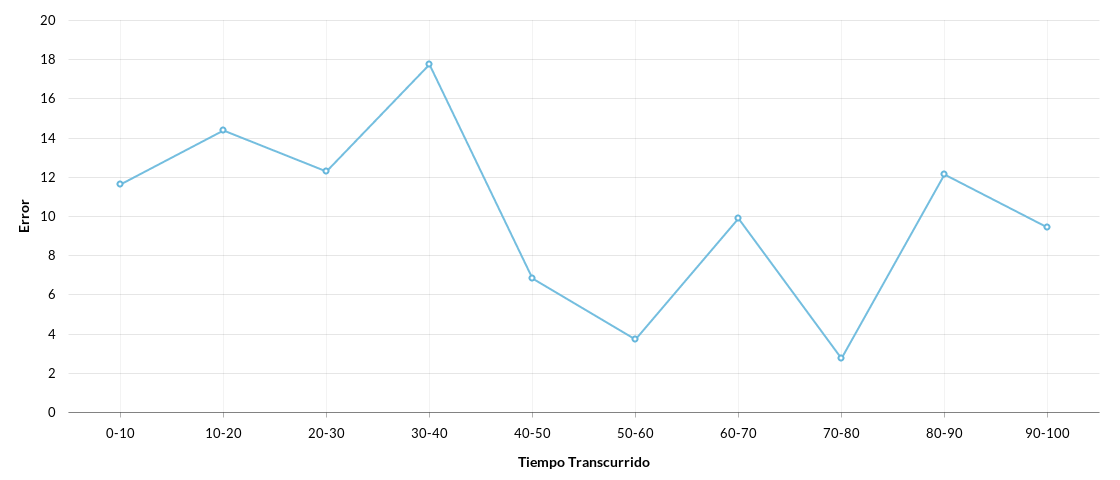
\includegraphics[width=0.8\linewidth]{./graphics/error_tiempo.png}
\caption{Distribuci\'on del Error Humano por Etapas de la Sesi\'on}
\label{figure:gerror-tiempo}
\end{figure}


\section{Encuesta}
\label{sec:resultados-encuesta}

Luego de haber finalizado la tarea cuatro, cada sujeto complet\'o una encuesta de manera tal a
opinar sobre su experiencia interactuando con el sistema de reconocimiento de voz. 
En la tabla~\ref{sec:tabla-encuesta} se puede observar un resumen de la encuesta realizada.


\begin{table}[H] 
\centering
\footnotesize
\begin{tabular}{|r|r|r|r|r|}
\hline
    Sujeto & Palabras & Comandos & Entrenamiento & Interfaz por Voz \\
    \hline
    1 & 6 & 7 & 6 & 7 \\
    2 & 6 & 7 & 7 & 7 \\
    3 & 7 & 7 & 7 & 7 \\
    4 & 6 & 6 & 4 & 5 \\
    5 & 7 & 7 & 7 & 4 \\
    6 & 6 & 6 & 5 & 5 \\
    7 & 7 & 7 & 7 & 5 \\
    8 & 6 & 7 & 6 & 7  \\
    9 & 6 & 7 & 7 & 5  \\
    10 & 5 & 6 & 6 & 6  \\
    11 & 6 & 6 & 6 & 7  \\
    12 & 6 & 6 & 7 & 5  \\
\hline
\end{tabular}
\caption{Resumen de la encuesta realizada.}
\label{sec:tabla-encuesta}
\end{table}

La figura ~\ref{figure:kiviat-encuesta1} presenta los valores promediados para cada columna
de la tabla anterior mediante un gr\'afico radial.

\begin{figure}[ht]
\centering
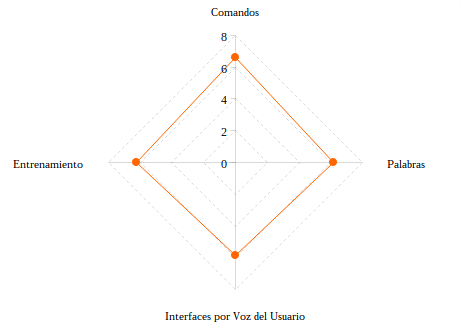
\includegraphics[width=0.6\linewidth]{./graphics/kiviat0.png}
\caption{Gr\'afico radial resumen de la encuesta realizada.}
\label{figure:kiviat-encuesta1}
\end{figure}

A continuaci\'on se presentan los resultados reescalados por usuario, en una escala del 0 al 1.


\begin{table}[H] 
\centering
\footnotesize
\begin{tabular}{|r|r|r|r|r|}
\hline
    Sujeto &  Palabras & Comandos & Entrenamiento & Interfaz por Voz \\
    \hline
1 &  0 & 1 & 0 & 1\\
2 &  0 & 1 & 1 & 1\\
3 &  - & - & - & -\\
4 &  1 & 1 & 0 & 0,5\\
5 &  1 & 1 & 1 & 0\\
6 &  1 & 1 & 0 & 0\\
7 &  1 & 1 & 1 & 0\\
8 &  0 & 1 & 0 & 1\\
9 &  0,5 & 1 & 1 & 0\\
10 & 0 & 1 & 1 & 1\\
11 & 0 & 0 & 0 & 1\\
12 & 0,5 & 0,5 & 1 & 0\\
\hline
\end{tabular}
\caption{Encuesta Reescalada.}
\label{sec:tabla-encuesta-normalizada}
\end{table}


La figura ~\ref{figure:kiviat-encuesta2} presenta los valores promediados para cada columna
de la tabla anterior mediante un gr\'afico radial. La misma permite observar el efecto del
cambio de escala, el cual facilita la identificaci\'on de fortalezas y debilidades. 

\begin{figure}[ht]
\centering
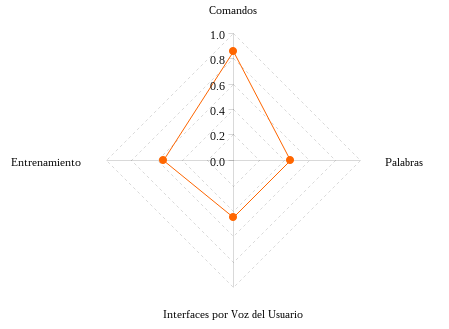
\includegraphics[width=0.6\linewidth]{./graphics/kiviat.png}
\caption{Gr\'afico radial resumen de la encuesta reescalada.}
\label{figure:kiviat-encuesta2}
\end{figure}
